%%%%%%%%%%%%%%%%%%%%%%%%%%%%%%%%%%%%%%%%%%%%%%%%%%%%%%%%%%%%%%%%%%%%%%%%%%%%%%%
%%%%%%%%%%%%%%%%%%%%%%%%%%%%%%%%%%%%%%%%%%%%%%%%%%%%%%%%%%%%%%%%%%%%%%%%%%%%%%%
%%
%%
%%             b.   M  E  T  H  O  D  O  L  O  G  Y  
%%
%%
%%%%%%%%%%%%%%%%%%%%%%%%%%%%%%%%%%%%%%%%%%%%%%%%%%%%%%%%%%%%%%%%%%%%%%%%%%%%%%%
%%%%%%%%%%%%%%%%%%%%%%%%%%%%%%%%%%%%%%%%%%%%%%%%%%%%%%%%%%%%%%%%%%%%%%%%%%%%%%%

\begin{figure}
  \begin{center}
   \hspace{-0.5cm}
%   trim=l b r t
    \includegraphics[width=16.0cm] %, trim={0.05cm 0 0.05cm 0},clip]
    {WP_overview.pdf}
    \vspace{-10pt}
  \caption{An overview of our WPs. {\bf N.B. Still needs a little updating}.}
  \vspace{-12pt}
 \label{fig:workplan}
\end{center}
\end{figure}
%% http://hubblesite.org/image/2012/news_release/2006-51
\section{Methodology}
%\noindent
%Here we describe our work plan in detail. We list our milestones and give the overall iteractions and workflow of the programme in Figure~1.
%
%\smallskip
%\smallskip
\noindent
This ERC Consolidator proposal kick starts the new field of Variable 
Extragalactic Astrophysics. Due to the Data Science aspect of this proposal, 
it is, at its heart interdisciplinary. 
%% 
We present a bold research vision that is designed to be addressed by
a research group, and the environment, current research areas and
telescope access at the Institute for Astronomy at the University of
Edinburgh is ideal to carry out these investigations.  The science
questions we seek to address are well-posed, yet strike at the heart
of major and still open extragalactic astrophysical questions: Do we
have a full accounting for the accretion history in the Universe?  How
does the energy `escape' from the central engine to the host galaxy?
Are the modes of AGN ``feedback'' that regulate a galaxy the same that
regulate the AGN itself?  What are the star-formation properties of
mid-infrared luminous quasars at the peak of quasar activity?

\smallskip
\smallskip
\noindent
Before laying out our Workplans, we make a note of the ethos involved in this project. 

\subsection{Project ethos}
\smallskip
\smallskip
\noindent
\textbf{\textsc{{Data Science and Observational Astrophysics: }}}
Data science is a new interdisciplinary field of scientific methods to
extract knowledge or insights from data in various forms, either
structured or unstructured. It employs techniques and theories drawn
from many fields within the broad areas of mathematics, statistics,
information science, and computer science, in particular from the
subdomains of machine learning, classification, cluster analysis, data
mining, databases, and visualization.  {\it Modern day observational
astrophysicists are in all but name data scientists, and as such, this
proposal is inherently interdisciplinary.}

\smallskip
\smallskip
\noindent
\textbf{\textsc{Breaking Down The Data Silos: }}
The bottleneck to using advanced data analysis is not skill base or
technology; it is simply access to the data.  A data silo is a
repository of fixed data that remains under the control of one
department/collaboration and is isolated from the rest of the world,
much like grain in a farm silo is closed off from outside
elements. These silos are isolated islands of data, and they make it
prohibitive to extract data and put it to other uses. In research
environments, and {\it especially in contemporary observational
astrophysics}, the data silos are open, but due to the lack of raw
person-power, still remain uncombined. The combination of P.I. and
host institute means we are uniquely positioned to break down these
astro-data silos for massively significant science gain.

\smallskip
\smallskip
\noindent
\textbf{\textsc{Targeting Big Data: }}
This ERC will develop and employ leadership-computing systems and
infrastructure to explore, prove, and improve a wide range of data
science techniques: uncertainty quantication; statistics; machine
learning; deep learning; databases; pattern recognition; image
processing; graph analytics; data mining; real-time data analysis; amd
complex and interactive workflows.

\smallskip
\smallskip
\noindent
\textbf{\textsc{Algorithms: }}
Our algorithms and methodology are based on the latest
machine-learning and data science
techniques. Specifically we will use 
\href{Python}{https://www.python.org/} as the CS-glue, 
\href{NumPy}{http://www.numpy.org/} for high-speed numerical processing, 
\href{pandas}{https://pandas.pydata.org/} for efficient data ingestion and 
\href{Matplotlib}{https://matplotlib.org/} for data visualization. 
%%
\href{http://ogrisel.github.io/scikit-learn.org/sklearn-tutorial/index.html}{\tt
scikit-learn} is a Python module integrating classic machine learning
algorithms in the scientific Python world (numpy, scipy,
matplotlib). It aims to provide simple and efficient solutions to
learning problems, accessible to everybody and reusable in various
contexts. Resources such as the
\href{https://github.com/jakevdp/PythonDataScienceHandbook}{{\tt
Python Data Science Handbook}} have full details. This includes the
``extreme deconvolution''
\href{http://www.sdss.org/dr14/data\_access/value-added-catalogs/?vac\_id=xdqso/}{`XDQSO'
technique}\footnote{\href{https://github.com/xdqso/xdqso}{\tt
github.com/xdqso/xdqso}}.



\smallskip
\smallskip
\noindent
\textbf{\textsc{Open Innovation, Open Science, Open to the World:}} 
The P.I. is an exceptionally strong, longtime and vocal supporter of
``Open Access''.  All my codes, data\footnote{Where I am not breaking
current data access agreements}, papers and proposals can be found at
\href{github.com/d80b2t}{{\tt github.com/d80b2t}}.  Indeed, this
proposal itself is now at that location.  One of the major research
outputs of this ERC will be computer code.  As such, we are already
working with the \href{The Software Sustainability Institute}{\tt
https://www.software.ac.uk/} which was founded to support the UK's
research software community.  Our software well be developed using the
FAIR ideology (Findable, Accessible, Interoperable,
Reusable\footnote{Wilkinson, MD, Sci Data. 2016 Mar 15;3:160018. doi:
10.1038/sdata.2016.18.})  and will be delivered in a manner which is
fully inline with ``Open Innovation, Open Science, Open to the
World''.



\subsection{Work Packages}
%\smallskip \smallskip \noindent {\bf  WORK  $\;$  PACKAGES} 
\smallskip 
\smallskip
\noindent
Our proposal contains six work packages that fall into three broad
and complementary categories: observational studies of large numbers
(millons) of objects; high-risk, very high-reward observational
studies of a small number (10s) of objects; theoretical modeling
investigations. Table 1 summarises our overall WP plan. Risks and
mitigation strategies are present for each WP as are Key Deliverables.

\smallskip
\smallskip
\noindent
We define three PDRAs, ``PDRA1'', ``PDRA 2'', ``PDRA 3'', and one PhD
student, ``PhD1''.  The skill set of PDRA1 would include development
of the underlying tools and techniques necessary to extract meaning
from large and/or complex data sets.  The skill sets of PDRA2 would
include expertise in time series analysis, primarily with optical
data but potentially also in other wavebands.  The skill set of PDRA3
would include experience with fluid mechanics modelling and/or large
computer simulations.  PhD1 would have a Masters or a strong 4-year
undergraduate degree in Physics or Mathematics with evidence of
research-level project work.

\medskip \medskip
\smallskip
\smallskip
\noindent
\textbf{\textsc{WP1: Build QuasarSieve:}} 

\smallskip
\smallskip
\noindent
Raw events come from LSST. The UK LSST Data Access Center (DAC, based
here at the University of Edinburgh) ingests this datastream and
re-emits a filtered stream. In order to utilize this filtered
datastream for our science goals we will build a ``Stage 2 filter'',
which we name {\it QuasarSieve}.  This second stage filter will
identify the quasars, add context, perform outburst forecasting etc.
Our light-curve algorithm will sit on top of {\it QuasarSieve} and
will trigger other telescopes to get e.g. timely spectrum or infrared
data.

\smallskip
\smallskip
\noindent
We will veto stars using ESA Gaia, the data of which are hosted by the
Wide-Field Astronomy Unit (WFAU) here at the Royal Observatory,
Edinburgh.

\smallskip
\smallskip
\noindent
The heavy-industry computing infrastructure is being supplied by the
LSST DAC and our task will be to build software in a timely and robust
manner.  This is a novel enterprise and a rate-limiting step in our
overal programme, with the associated high-risk.  We mitigate this
risk with the data science and machine learning experience from PDRA1
and the P.I. (NPR).  We will also mitigate risk by taking advantage of
the algorithm resources and LSST DAC staff, here at the Royal
Observatory, Edinburgh.  We thus classify {\bf WP1 as medium-risk,
high-reward.}  {\bf Key Deliverables:} An open-source, well-documented
software package that can interact with and return data from the LSST
Data Access Center.



\medskip 
\medskip
\smallskip
\smallskip
\noindent
\textbf{\textsc{WP2: Quasar Catalogue Generation and Demographic studies:}}  

\smallskip
\smallskip
\noindent
Building the quasar corpus and cataloguing the observational data will
be a vital step in beginning to pursue our science goals. This
catalogue will be the glue that binds the observational projects
together and will have not only the data, but also the metadata to
enable the other WPs.  Following on from the quasar catalogue
generation, a key science output will be the study of the quasar
demographics.  Luminosity function, clustering and higher-order
statistics will be made in order to precisely determine the census of
quasars, their environments, their host galaxy preferences and their
evolution. All these are vital observational tests for galaxy
formation models and theory (see WP4 below). The goal of this WP is to
construct a quasar catalogue and make key observational tests.
Given the P.I.s experience at these specific tasks, plus the effort
level of PDRA1, PDRA2 and PhD this WP is deemed medium-risk.

\smallskip
\smallskip
\noindent
{\bf WP2 is medium-risk, high-reward.}  {\bf Key Deliverables:} A
science-enabling compendium that will be the state-of-the-art quasar
dataset for the 2020s.  A suite of new, beyond-the-state-of-the-art
quasar demographic measurements which are the boundary conditions for
theoretical models.

\begin{figure}[h]
  \begin{center}
   \hspace{-0.5cm}
%   trim=l b r t
    \includegraphics[width=16.0cm] %, trim={0.05cm 0 0.05cm 0},clip]
%   {figures/Angles-Alcazar_2013_fig5.pdf}
   {figures/Angles-Alcazar_2013_fig7.pdf}
    \vspace{-10pt}
   \caption{
\footnotesize 
Two theoretical models from \citet{Angles-Alcazar2013} with different
accretion modes.  From top to bottom: (1) total (stellar and gas) disk
mass evaluated within $R_{0} = 1$ kpc, (2) total disk mass fraction
within $R_{0}$ , (3) ratio of gas mass to total (stellar and gas) disk
mass evaluated at $R_{0}$ (solid line), provided that $f_{\rm gas}
\geq f_{0}$ (dashed line) inflow rates are not limited by gas supply,
and (4) inferred black hole accretion rates using the analytic model
of \citet{Hopkins_Quataert2011} (Equation (2)), where we have used a
constant black hole mass $M_{\rm BH} = 10^{5} M_{\odot}$ at all times
and normalized to the peak accretion rate.
}
  \vspace{-18pt}
 \label{fig:ERQ}
\end{center}
\end{figure}

\medskip 
\medskip
\smallskip
\smallskip
\noindent
\textbf{\textsc{WP3: Light-Curve and Spectral Analyses:}} 

\smallskip
\smallskip
\noindent
Another major scientific output that will originate from the quasar
corpus catalogue generation will be the full and detailed light-curve
and spectral analyses of the said catalogue. This will result in the
discovery of light-curve trends with quasar type, new methods to
measure black hole mass and the key science goal to see which quasars
are ``changing-look'' objects. This WP will have a data
science/machine learning aspect.  The goal of this WP is to elucidate
the physical processes that drive quasar variability.  The full
Light-Curve and Spectral Analyses that we envisaged will be a
significant amount of work, leading to significant high-reward
science.  


\smallskip
\smallskip
\noindent
{\bf WP3 is medium-risk, high-reward.}  
This level of investigation is highly novel, though we envisage no
major barriers outside of our control to achieving our science goals
and PDRA1, PDRA2, as well as the P.I. (NPR) and PhD1 effort will be
directed towards this.
As such, we deem this medium-risk.  {\bf Key Deliverables:}
Measurements, for the first time of how the light-curves and spectra
of quasars depend on key physical quasar properties e.g. $M_{\rm
SMBH}$, luminosity, $\lambda = \log (L / L_{\rm Edd})$, spin etc.
These measurements will allow us to make direct comparisons to
accretion disk models.



\medskip 
\medskip
\smallskip
\smallskip
\noindent
\textbf{\textsc{WP4: Accretion Disk and Quasar Feedback Simulations:}} 

\smallskip
\smallskip
\noindent
New accretion models are needed to fully explain the observational
data of ``changing look'' quasars that we have examples of today and
the ``Quasar Viscosity Crisis''. New radiation MHD codes begin to
explain the observations here, but further development is needed to
gain the desired deep understanding. Cosmological-scale hydrodynamic
simulations with stellar and quasar feedbasck are now also online. The
exceedingly ambitious goal of WP5 is to develop new holistic accretion
disk-to-cosmological scale simulations that explain our observational
results and link them to ``quasar feedback''.  WP4 is thus high-risk
due to its novel nature and algorithmic complexity.  We also envisage
ramp-up time to get our theoretical simulations to the level that will
be required by our beyond-the-state-of-the-art dataset.  However, we
mitigate this risk first by noting this will be the lead WP and top
priority for PDRA3.  We further mitigate this risk by invoking
collaboration with accretion disk theorist Prof. Ken Rice (WKMR; Chair
of Computational Astrophysics at the IfA, University of Edinburgh) and
Prof. Romeel Dave (RSD; Chair of Physics in the IfA, University of
Edinburgh).

\smallskip
\smallskip
\noindent
Thus PDRA3, NPR, potentially PDRA2, with guidance where nesceassy from
WKMR and RSD would collaborate on this WP.  We thus classify {\bf WP4
as medium-to-high risk, very high-reward.}  {\bf Key Deliverables:}
New accretion disk models and theory that explain the light curve data
of our beyond-the-state-of-the-art dataset.  New galaxy evolution
models, describing the hydrodynamics involved on galactic scales, but
related to the quasar central engine.



\begin{figure}[h]
  \begin{center}
%   \hspace{-0.5cm}
%   trim=l b r t
    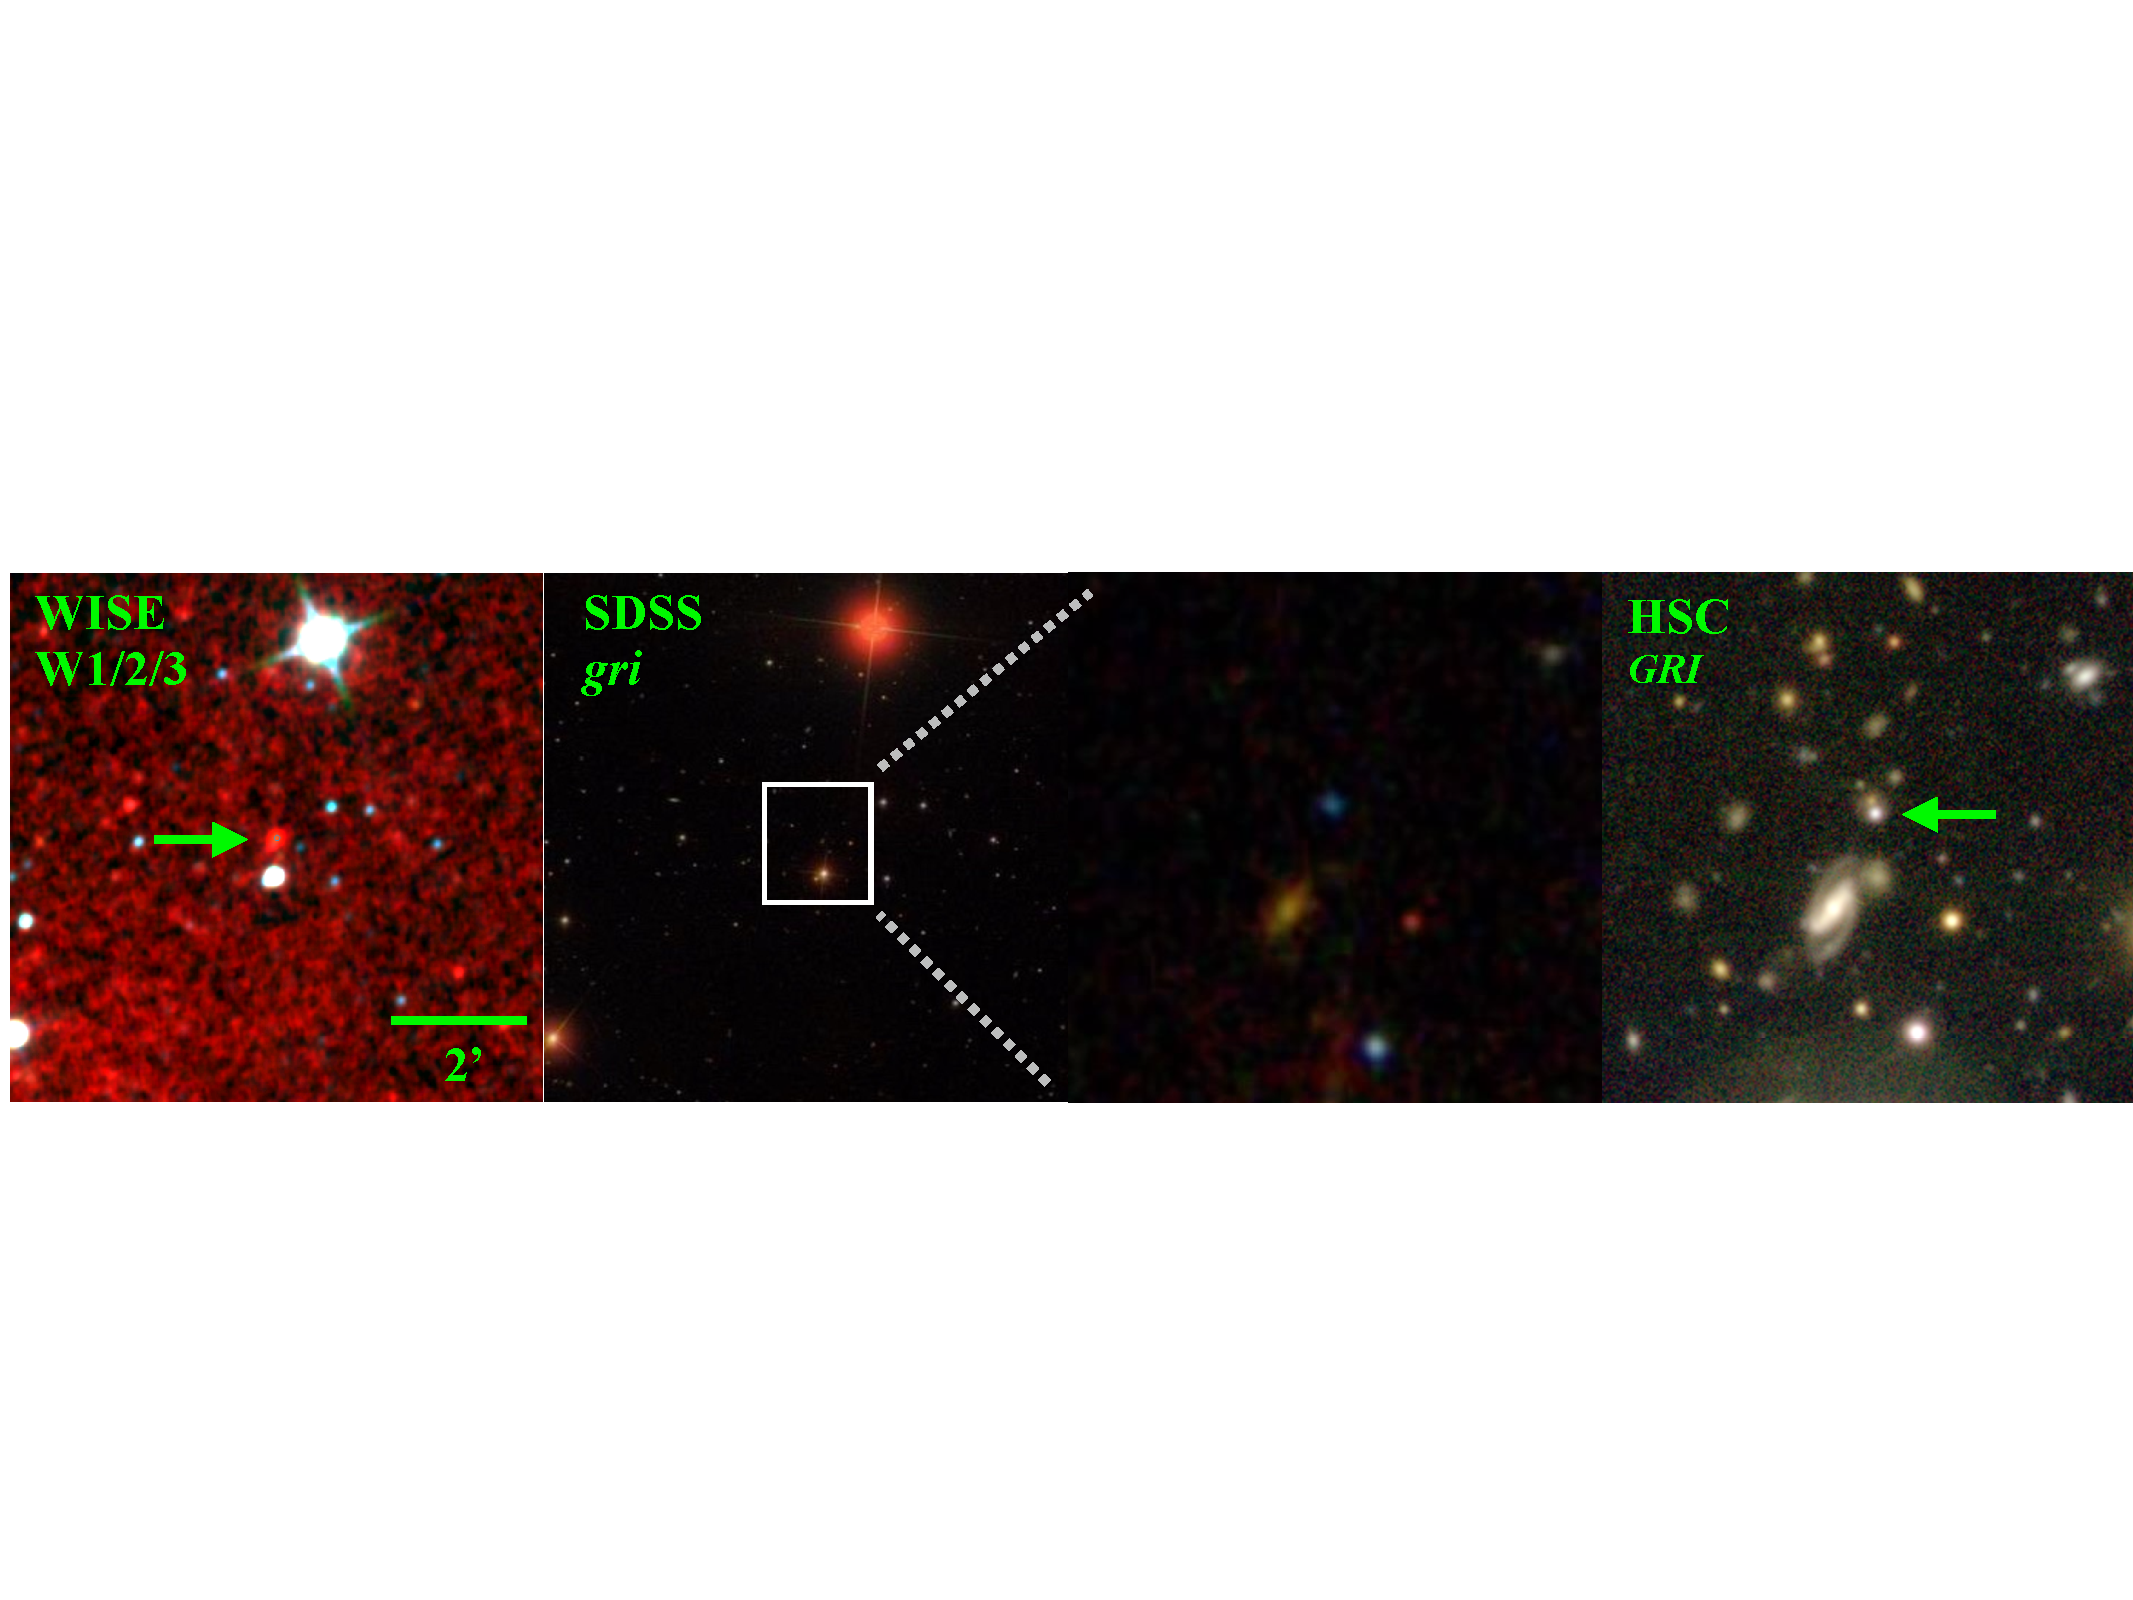
\includegraphics[width=17.0cm, trim={0.15cm 0 0.05cm 0},clip]
   {figures/WISE_SDSSzoomHSC_ERQ-image_v3.pdf}
    \vspace{-20pt}
   \caption{%\small   
\footnotesize 
%     \scriptsize
 %    \tiny
The IR and optical imaging of J2323-0100, an archetype of the
``Extremely Red Quasars'' (ERQs) at $z\approx2.5$ and a {\it JWST}
target. Shown are WISE {\it (left)}, where the quasar booms out as
indicated by the arrow; the SDSS image {\it (middle left)} with
zoom-in {\it (middle right)} on the optically faint source, and new
HSC imaging {\it (right)}, which shows tantalizing evidence for a
faint companion galaxy. Optical rest-frame spectra of J2323-0100,
revealed very broad (FWHM = 2500-5000 km s$^{-1}$), strongly
blue-shifted (by up to 1500 km s$^{-1}$) \oiii\ $\lambda$5007\AA\
emission lines in the ERQs. This is suggestive of active outflows and
potentially evidence for AGN feedback in action at the height of SMBH
activity.
}
  \vspace{-12pt}
 \label{fig:ERQ}
\end{center}
\end{figure}

\medskip
\medskip
\smallskip
\smallskip
\noindent
\textbf{\textsc{WP5: Observations of Quasars by the James Webb Space Telescope}} 

\smallskip
\smallskip
\noindent
In \citet{Ross2015} I discovered a new class of object, the ``extremely red
quasars'', that have optical spectroscopy from SDSS/BOSS, and
$r-[22\mu{\rm m}]>14$ colors (i.e., $F_{\nu,\, {\rm MIR}} / F_{\nu,\,
{\rm opt}} \gtrsim 1000$) from the Wide-field Infrared Survey Explorer
(WISE; [17]) satellite, see Figure~\ref{fig:ERQ}.  The ERQs are a
unique obscured quasar population with extreme physical conditions
related to powerful outflows across the line-forming regions. These
sources are the signposts of the most dramatic form of quasar feedback
at the peak epoch of galaxy formation, and may represent an active
``blow-out'' phase of quasar evolution ([18], [19]).  However, due to
the current lack of access to mid-infrared spectroscopy, it is still
unknown whether the large IR luminosities observed in these quasars is
from star formation, which would produce strong polycyclic aromatic
hydrocarbon (PAH) spectral features, or, if it is from the hot dust
near the central quasar, which should produce much weaker/no PAH
emission.

\smallskip
\smallskip
\noindent
What are the star-formation properties of luminous quasars at the peak
of quasar activity?  We aim to answer this by looking for the presence
of polycyclic aromatic hydrocarbon (PAH) spectral features in infrared
bright quasars with the {\it James Webb Space Telescope} (JWST).  

\smallskip
\smallskip
\noindent
{\bf WP5 is high risk, high-reward.}  This is an ideal investigation for
the JWST, but we classify this as high-risk since we have to apply for
the telescope time and are not guaranteed the data.  We note this will
be the single WP NPR would lead and does not impact in any direct way
the other WPs. This would lead to very-high gain science.  {\bf Key
Deliverables:} State-of-the-art data products from the JWST, with the
observational evidence and physical interpretation of how ``quasar
feedback'' regulates galaxy formation in high-redshift quasars.

\smallskip
\smallskip
\noindent
{\bf WP5 is medium-to-high risk, high-reward.}
This is an ideal investigation for the James Webb Space Telescope, but we classify this as `high-risk' since this is the one telescope/survey/mission where we would have to bid/apply for the telescope time and are not guaranteed the data. We mitigate the risk here by saying that this will be the one project the P.I. (NPR) would directly lead, and would lead to very-high gain science, but does not impact in any direct way any of the other WPs. 



%%%
%%%   W P   6 
%%%
\medskip
\medskip
\smallskip
\smallskip
\noindent
\textbf{\textsc{WP6: New Object Discovery:}} 

\smallskip
\smallskip
\noindent
The LSST will scan the sky repeatedly, enabling it, and us, to both
discover new, distant transient events and to study variable objects
throughout our universe. The LSST will extend our view of the
changeable universe a thousand times over current surveys.  The most
interesting science to come may well be the discovery of new classes
of objects.

\smallskip
\smallskip
\noindent
{\bf WP6 is medium-risk, exceptionally high-reward.}  We class this as
medium-risk, since it is tricky to class a WP with essentially unknown
discovery potential as fully `low-risk'. However, we do not classify
this as `high-risk' since if there was a paucity of discovery of novel
classes of objects, this would be the first time in the hitorsy of
observational astrophysics that a new facility such as LSST has come
online and found nothing new.  {\bf Key Deliverables:} Potential
discovery of new classes of astronomical objects.



\medskip  \medskip \smallskip \smallskip \noindent
\subsection{Feasibility}

\smallskip
\smallskip
\noindent
By its inherent nature, our programme is high-risk and high-reward, but
we {\it fundamentally} have the personnel and skill sets that are 
necessary to make this project feasible. 
%% Mention your experience and knowledge to hedge against this risk or alternative approaches or help from collaborators. 
The P.I. has a track-record of managing scientific groups in 
large international and world-leading collaborations. {\it Critically, 
he also has a track record of developing key software packages 
on strict deadlines, e.g. the BOSS Quasar Target Selection software 
package (that contained a suite of novel ML algorithms).}
%
%% Have a dedicated section on feasibility of what you are proposing. Explain which WP’s/tasks present high levels of risk. 
%
%%Provide a contingency plan, particularly if any of the tasks are unconventional, present a great challenge and are high risk (but also high gain). 

%
%% Be ``safely adventurous''.  
%
%% Include a gantt chart or a timeline for the evaluators to visualise the timescale of each component of the work you are proposing.  Include a 4-5 line summary to recap and remind the evaluator what the essence of the project is and why it so important to get this funded now.




